\section{Sentiment Analysis}
\label{chap:sent}
As stated in \citep{Veselovska}: "Sentiment analysis, also known as opinion mining, is an automatic detection of a positive or negative polarity, or neutrality of ... a text sequence", which is exactly as the sentiment analysis is understood in this work, although there are some other definitions consisting of e.g. opinion extraction, irony or stance \citep{Montoyo2012} and sentiment analysis can also continue with e.g., opinion extraction. Another tasks related to sentiment analysis is a subjectivity analysis (whether the presented opinion is objective or highly subjective), which is also not included in this work, mainly because the lack of labelled data for Czech. It is possible to analyze individual expressions, sentences or whole documents \citep{Veselovska}. This thesis focuses on the document-level classification, which has many real-life use cases and Czech training data are available.
\subsection{Task definition}
\paragraph{Sentiment analysis} \mbox{}\\
\textit{input:} sequence of sentences (a whole post or comment, depending on the source) \\
\textit{output:} prevailing sentiment of the input from categories: neutral, positive, negative.
\par


%TODO zero experiments
\paragraph{Metric} For evaluating performance, two metrics are used: weighted-F1 score and accuracy. Accuracy is a standard metric for classification and weighted-F1 allows better comparability and also provides additional insights into models evaluation.

\subsection{Related Work}
As every languge-related task, sentiment analysis is best explored for English. It is possible to derive sentiment by supervised learning (typical are Support Vector Machines or Maximum Entropy classifier) or using rule-based approach -- vocabulary of emotionally coloured words, emoticons etc \citep{Cano2019}, \citep{Veselovska}. BERT-like models were succesfully used to improve result for sentiment analysis task on English \citep{Devlin2019} and also other languages, for example Estonian \citep{Kittask2020}, Indonesian \citep{putra} or Italian \citep{pota2021effective}.
\par
There are not so many attempts to sentiment analysis in Czech in comparison to English, however some attempts were made with both neural networks and traditional machine learning - naive bayes classifiers, support vector machines, and maximum-entropy-based classifiers \citep{Veselovska}.  A thorough study of supervised machine learning methods on \textit{mall} and \textit{facebook} dataset is offered in \citep{Cano2019}. For a practical use, \citep{Zizka} presented automatic sentiment prediction of unlabelled text based on a small set of labelled patterns via searching similarities. As the neural networks dominates in many NLP taks, they are also applied in sentiment analysis. One of first attepts to apply neural networks on Czech sentiment is described in \citep{Lenc}, which evaluates besides others all three datasets used in this work on document-level sentiment analysis. \citep{kysely} performes sentiment analysis using embeddings and convolutional neural network on multidimensional embedding, which is quite unusual as CNNs are typically used for image processing. \citep{kysely} uses same three datasets, but classifies only on sentence-level (they filtered out longer samples), which is simpler as longer texts tend to be more inconsistent about sentiment \citep{Veselovska}. \citep{Libovicky} presents state-of-the art results in three czech NLP tasks including sentiment analysis. They use only CSFD dataset with resulting accuracy 80.8\% which is comparable to previous \acrshort{sota} \citep{Brychcin2013}. The second mentioned paper uses quite complicated method for classification incorporating the fact of which movie is reviewed, while \citep{Libovicky} uses only bidirectional LSTMs with multiple attention heads following state-of-the-art results on English \citep{Lin2017}. There are five previous works know to me, which involves BERT-like models in Czech sentiment: 
\begin{itemize}
\item XLM-Roberta applied on all three datastets trimmed to 128 characters \footnote{http://www.janpalasek.com/sentiment-analysis-czech.html}
\item \citep{Klouda} applies multilingual BERT on mall dataset with resulting accuracy about  81\%, which did not outperform the naive bayes classifier baseline with 84\% accuracy, 
\item  \citep{Sido2021} presents monolingual Czech model Czert,  based on BERT and ALBERT models, and evalutes it on csfd and facebook datastets with new state-of-the-art results,
\item \citep{Straka2021} published another monolingual model, based on more succesfull RoBERTa model and surpassed Czert on facebook dataset.
\end{itemize}

\subsection{Dataset and Preprocessing}
%TODO habernal vytvoril ty datasty 
%TODO zjistit jaka jsou na to porovnavaci data This work primary tries to improve existing tasks and show the ability of contextualized embeddings to improve results, so tasks with existing data and results were selected.  %TODO why?
Four main Czech datasets with sentiment annotation are available: news from Aktualne.cz (aktualne) \citep{Veselovska}, user reviews from MALL.cz (mall), film reviews from csfd.cz (csfd), and posts from Czech branch pages on facebook.cz (facebook) (last tree in \citep{Habernal.et.al.2013}). As \textit{aktualne} dataset turned out to be problematical because the text were ambiguous even for annotators, and its authors later used other mentioned datasets \citep{Veselovska}, this work also focuses only on the three other data sources -- \textit{mall}, \textit{csfd} and \textit{facebook} \footnote{All three datasets are all available here: http://liks.fav.zcu.cz/sentiment/}. Some experiment are also performed with in-domain training on English data. For this purpose is used \textit{imdb} dataset, \footnote{https://www.tensorflow.org/datasets/catalog/imdb\_reviews} which contains movie reviews from the biggest movie rating website imdb.com. This leads to some problems described later in this section, because English dataset contains only binary classification (positive/negative). Table \ref{tab:datasets} summarize each dataset. All dataset were randomly split into train, development and test datasets with the same labels distribution as original datasets.
\par
\begin{figure}[!h]
\centering
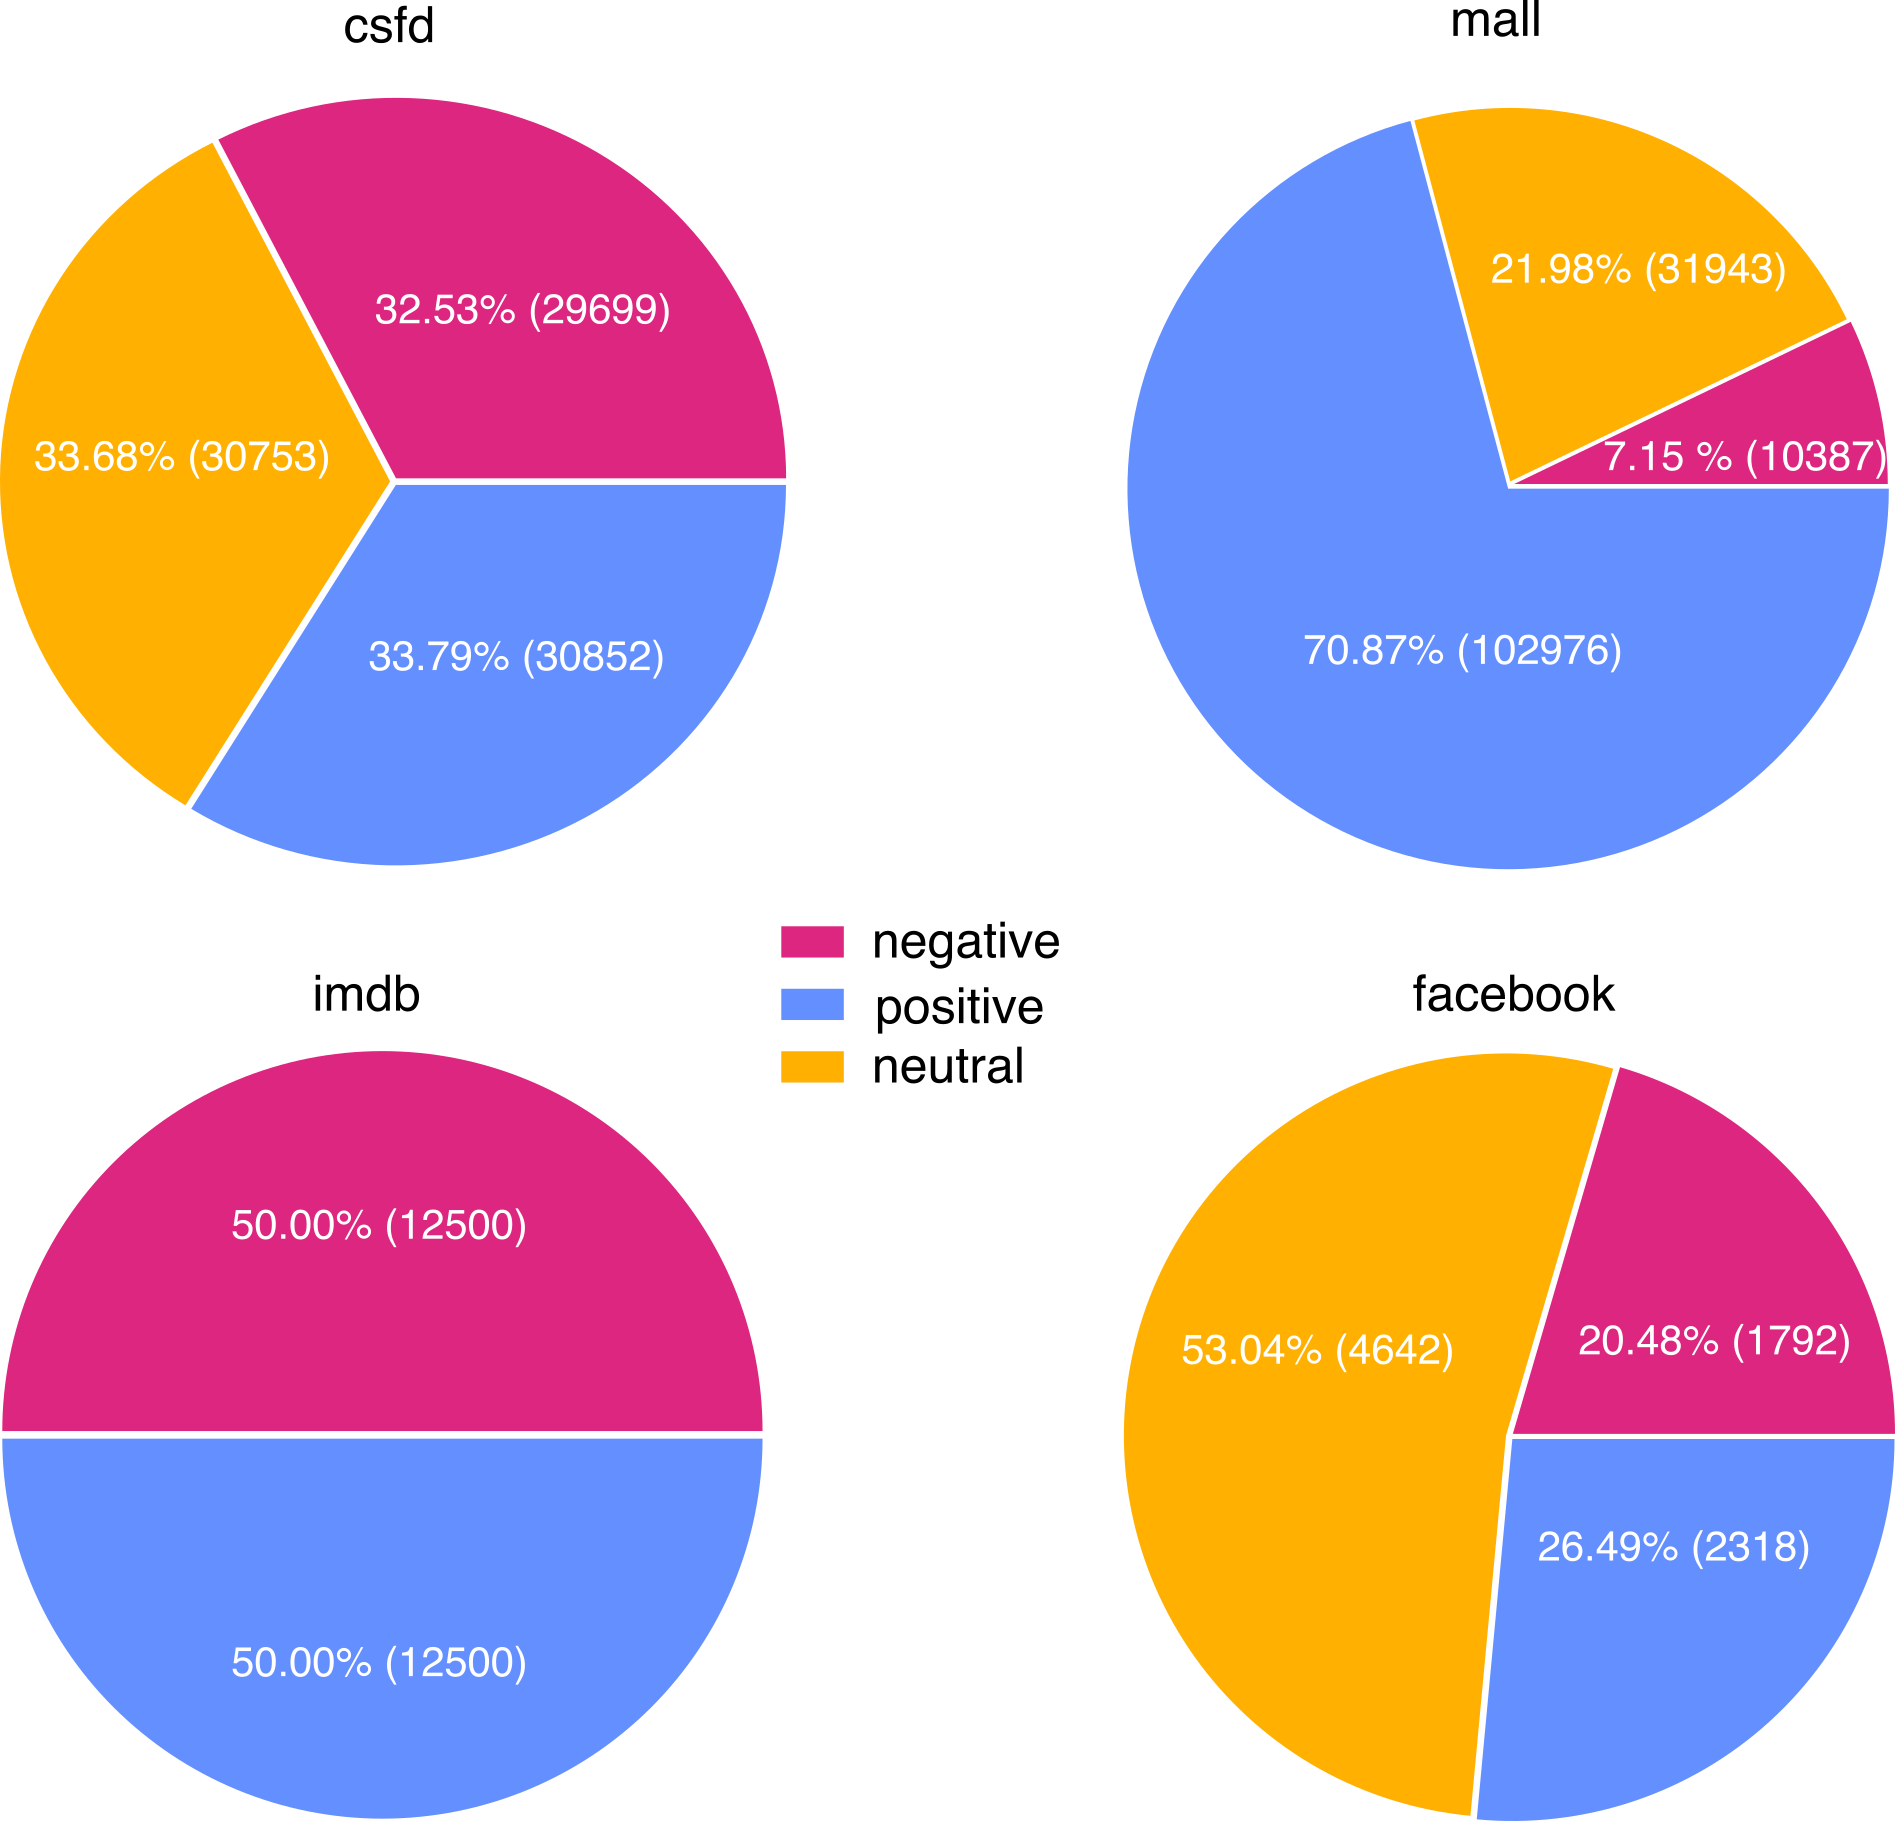
\includegraphics[width=0.95\columnwidth]{../img/dist_all.png}
\protect\caption{Distribution of positive/neutral/negative labels in each dataset.}
\label{pic:dist}
\end{figure}

\begin{figure}[!h]
\centering
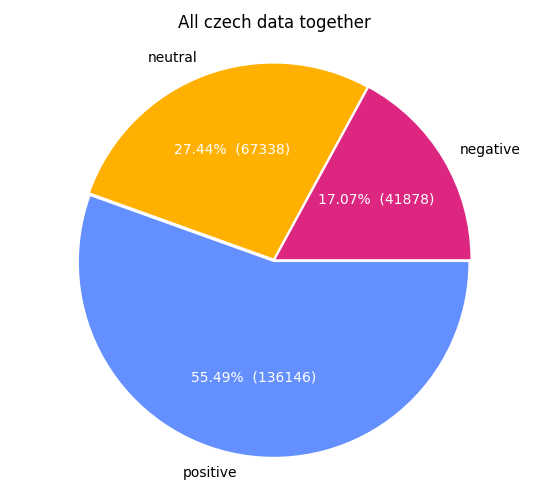
\includegraphics[width=0.65\columnwidth]{../img/all.png}
\protect\caption{Percentage and absolute values of labels in all three Czech datasets together.}
\label{pic:dist_all}
\end{figure}
As can be seen in figure \ref{pic:dist}, distribution of labels differs among datasets. Moreover, Figure \ref{pic:dist_all} shows, that the resulting dataset is highly unbalanced, which may causes divergence and stuck in training. Due to the big part of labels being positive, many learning strategies just ended with predicting only \textit{positive} class, i.e. 55\% accuracy, so unfortunately learned nothing. 
\begin{center}
\begin{table}[!h]
\begin{tabular}{|l||lll|}
\hline
     & length & labels                                                                & domain        \\ \hline \hline
\textbf{mall}     & 145306 & \begin{tabular}[c]{@{}l@{}}positive\\ neutral\\ negative\end{tabular} & domestic appliance reviews                             \\ \hline
\textbf{csfd} & 91304  & \begin{tabular}[c]{@{}l@{}}positive\\ neutral\\ negative\end{tabular} & movie reviews \\ \hline
\textbf{facebook} & 9752   & \begin{tabular}[c]{@{}l@{}}positive\\ neutral\\ negative\end{tabular} & \begin{tabular}[c]{@{}l@{}}brand pages of e.g. shops or mobile network\\ providers\end{tabular} \\ \hline
\textbf{imdb} & 25000  & \begin{tabular}[c]{@{}l@{}}positive\\ negative\end{tabular}           & movie reviews \\ \hline
\end{tabular}
\caption{Three Czech datasets (mall, facebook, csfd) and one English (imdb) are used for training in this work.}
\label{tab:datasets}
\end{table}
\end{center}

\subsection{Experiments and Architecture}
The main division of experiments is by the input dataset -- each of Czech models separately and one joint dataset consisting of all Czech datasets, i.e. four different datasets. All variants performed both layers attention and an average of last four layers. As for the learning rate, all experiments were made with learning rate $3 \times 10^{-5}$ and there were always two types of learning rate decay -- cosine and inverse square root decay. 
\par
Network architecture is much simpler than in tagging and lemmatization task and corresponds to \textit{simple} setting of these tasks -- only BERT-like model and classification head consisting of layer with softmax activation function. 
\par 
Baseline for these models is Naive Bayes Classifer (NB) with term frequency--inverse document frequency (tf--idf) representation. \textit{tf\_idf}-s for each word are defined in this way: \textit{tf} stands for a term frequency
\[ tf = \frac{word\_occurences}{number\_of\_words\_in\_document} \]
and this is count over the whole dataset, while \textit{idf} is inverse document frequency
\[idf = \frac{number\_of\_documents}{number\_of\_documents\_with\_word}.\]\textit{Idf} works as an evaluation of the importance of the word. The result is then: \[tf\_idf = tf \cdot idf .\] 
This representation serves as an input into Naive Bayes Classifier (NB). NB \citep{duda1973pattern} is a probabilistic model, which models probability of the class $k$ given the data features $x_i$: $p(C_k|x_1,...,x_n)$ and uses \textit{naive} assumption of features to be independent. 

\subsection{Results and Discussion}
Models based upon RoBECzech not only outperformed baseline, but also achieved new state-of-the-art results in all three datasets as can be seen in table \ref{tab:res_sent_best}. Complete results can be seen in table \ref{tab:res_all_sent}. The best model for each dataset was the one trained on that dataset, although model trained on joint datasets performed comparable to single-data model on \textit{csfd} and \textit{mall}. For \textit{facebook}, joint model was worse by 9\%. This can be caused by the a difference in distribution of labels between datasets. \textit{Facebook} dataset has the most different label distribution in comparison to \textit{all\_czech} together (mostly neutral posts vs. mostly positive, see Fig. \ref{pic:dist} and Fig. \ref{pic:dist_all}). 

%TODO sjednotit jmeno spolecneho datasetu

%TODO chyba v predikci, prohozeni
%mall: outputs/0608-2341_sent_o_63 , 'sentiment_analysis.py-2021-06-08_234151-a=12,bs=4,b=..'
%facebook: 'sentiment_analysis.py-2021-06-08_172844-a=12,bs=4,b=..'
%csfd: sentiment_analysis.py-2021-07-05_115521-a=16,bs=2,b=..
%bezi mi join

%TODO pusten mall

%TODO napsat proc to neni crossvalidovane a ze ty cisla tedy jsou divna, pusteno s tremi ruznymi seedy tak pak udelam prumer
%TODO 16 pusteno na 10 epoch - stale bezi, stale bezi
%TODO habernal limity accuracy a oduvodneni v kysely



\begin{table}[!h]
\centering
\begin{tabular}{|l|l||ll|}
\hline
dataset                    & models      & Acc   & F1    \\ \hline \hline
\multirow{5}{*}{All Czech} & baseline    & 82.00 & 70.00 \\ \cline{2-4} 
                           
                           
                           
                           & \textit{\citep{kysely}} & \textit{67.82} & \textit{67.00} \\ \cline{2-4}
                           & best(16)    & \textbf{84.04} & \textbf{84.86} \\ \hline \hline
\multirow{3}{*}{csfd}      & baseline    & 69.07 & 69.00 \\ \cline{2-4} 
& \textit{Czert}       &       & \textit{84.79} \\ \cline{2-4} 
& $\textit{\citep{kysely}}\star$ & \textit{71.34} & \textit{71.00} \\ \cline{2-4}
                           & best(16)    & 84.02 & 84.00\\ \cline{2-4} 
                           & best(69)    & \textbf{84.89 }& \textbf{84.87} \\ \hline \hline
\multirow{3}{*}{mall}      & baseline    & 84.72 & 83.00 \\ \cline{2-4} 
& \textit{\citep{kysely}} & \textit{82.52} & \textit{81.00} \\ \cline{2-4}
& \textit{\citep{Klouda}} & 81.00 & 79.00 \\ \cline{2-4}
                           & best(16)    & 84.40 & 84.00 \\ \cline{2-4} 
                           & best(63)    & \textbf{84.60} & \textbf{84.14} \\ \hline \hline
\multirow{3}{*}{facebook}  & baseline    & 67.30 & 63.00 \\ \cline{2-4} 
& \textit{RobeCzech }  &       & \textit{80.13} \\ \cline{2-4} 
& \textit{XLM-RoBERTa} &       & \textit{82.29} \\ \cline{2-4} 
& \textit{Czert}       &       & \textit{76.55} \\ \cline{2-4} 
& \textit{\citep{kysely}} & \textit{71.62} & \textit{71.00} \\ \cline{2-4}
                           & best(16)    & 75.00 & 74.98 \\ \cline{2-4} 
                           & best(45)    & \textbf{81.80} & \textbf{81.65} \\ \hline
\end{tabular}
\caption{Best results for all datasets and a comparison to previous work. Best(16) is a best model for joint dataset and best(x) is always the best model for respective dataset. Numbers in italics are from related work. \protected\\ $\star$ \citep{kysely} performs only sentence-level classification. }
\label{tab:res_sent_best}
\end{table}

\begin{table}[!h]
\centering
\begin{tabular}{|l||c|c|c|c|}
\hline
 Input &
  joint &
  mall &
  facebook & csfd \\ \hline \hline
\begin{tabular}[c]{@{}l@{}}Rozbila se po prvním použití, je na hovno.\\ \textit{It broke after the first use, it is shitty.}\end{tabular} &
  \cellcolor[HTML]{648FFF}Neg &
  \cellcolor[HTML]{648FFF}Neg &
  \cellcolor[HTML]{648FFF}Neg & 
  \cellcolor[HTML]{DC267F}Neut\\ \hline
\begin{tabular}[c]{@{}l@{}}Rozbila se až za rok.\\ \textit{It broke after a year of use.}\end{tabular} &
  \cellcolor[HTML]{648FFF}Neg &
  \cellcolor[HTML]{648FFF}Neg &
  \cellcolor[HTML]{648FFF}Neg & 
  \cellcolor[HTML]{DC267F}Neut\\ \hline
\begin{tabular}[c]{@{}l@{}}S manželem jsme si víkend moc užili.\\ \textit{Me and my husband enjoyed the weekend.}\end{tabular} &
  \cellcolor[HTML]{FFB000}Pos &
  \cellcolor[HTML]{FFB000}Pos &
  \cellcolor[HTML]{FFB000}Pos & 
  \cellcolor[HTML]{FFB000}Pos \\ \hline
\begin{tabular}[c]{@{}l@{}}Ok, ale nic zajímavého.\\ \textit{Ok, but nothing interesting}.\end{tabular} &
  \cellcolor[HTML]{DC267F}Neut &
  \cellcolor[HTML]{648FFF}Neg &
  \cellcolor[HTML]{648FFF}Neg &
   \cellcolor[HTML]{648FFF}Neg \\ \hline
\begin{tabular}[c]{@{}l@{}}super zboží \\ \textit{super product}.\end{tabular} &
  \cellcolor[HTML]{FFB000}Pos &
  \cellcolor[HTML]{FFB000}Pos &
  \cellcolor[HTML]{FFB000}Pos &
  \cellcolor[HTML]{DC267F}Neut \\ \hline
\end{tabular}
\caption{Evaluation of models on four Czech sentences. \textit{mall} model was not included as a separate option, as the best model is the joint one.}
\label{tab:four_sent}
\end{table}
%TODO oznacit sotas nejakym symbolem
Following \citep{kysely}, resulting models were evaluated on five different czech sentences to manifest the differences between models (Table \ref{tab:four_sent}). It can be seen that predicting neutral vs. negative is still tricky for models, which can be also seen in confusion matrices \ref{tab:conf}. Confusion matrices shows, that predicting neutral is complicated in general, meanwhile models have learned to distinguish well between positive and negative sentiment.  Table \ref{tab:four_sent} also shows that \textit{csfd} model is quite different from the rest. It is probably caused by the difference in the training data nature. 

\begin{table}[!h]
\centering
\begin{tabular}{|llllll||llll|}
\hline
\multicolumn{5}{|c}{Combined datasets (16)}                          &  & \multicolumn{4}{c|}{mall (63)}        \\
                             & \multicolumn{4}{c}{predicted labels} &  & \multicolumn{4}{c|}{predicted labels} \\
\multirow{4}{*}{\rotatebox[origin=c]{90}{True labels}} &         & neut    & neg    & pos     &  &         & neut    & neg     & pos   \\
                             & neut    & 7027    & 885    & 2025    &  & neut    & 2896    & 199     & 1696   \\
                             & neg     & 1122    & 4783   & 307     &  & neg    & 344     & 1082    & 132    \\
                             & pos     & 1279    & 207    & 18857   &  & pos     & 932     & 54      & 14461  \\ &&&&&&&&&\\ \hline \hline
\multicolumn{5}{|c}{csfd (69)}                                       &  & \multicolumn{4}{c|}{facebook (45)}    \\
\multirow{4}{*}{\rotatebox[origin=c]{90}{True labels}} &         & neut    & neg    & pos     &  &         & neut    & neg      & pos   \\
                             & neut    & 3600    & 685    & 170     &  & neut    & 440     & 41       & 51    \\
                             & neg     & 603     & 3769   & 241     &  & neg     & 57      & 135      & 7     \\
                             & pos     & 146     & 225    & 4257    &  & pos     & 23      & 3        & 243  \\ &&&&&&&&& \\ \hline
\end{tabular}
\caption{Confusion matrices for best model in each category.}
\label{tab:conf}
\end{table}


%TODO tady mam best pro ruzne datasety a neni to uplne porovnatene

% Please add the following required packages to your document preamble:
% \usepackage{multirow}
\begin{table}[]
\centering
\resizebox*{!}{\textheight-2pt}{\begin{tabular}{|l|l|l|l||ll|}
\hline
\multicolumn{2}{|l|}{MODEL}       & EXPE                      & LRTYPE                & Acc    & F1   \\ \hline  \hline
1  & \multirow{6}{*}{mBERT}     & czech                     & \multirow{3}{*}{Isrd} & 80.89   & 80.62 \\ \cline{1-1} \cline{3-3} \cline{5-6}
2  &                            & zero                      &                       & 49.51   & 44.67 \\ \cline{1-1} \cline{3-3} \cline{5-6}
3  &                            & eng                       &                       & 81.17   & 80.90 \\ \cline{1-1} \cline{3-6}
4  &                            & czech                     & \multirow{3}{*}{cos}  & 82.56   & 82.35 \\ \cline{1-1} \cline{3-3} \cline{5-6}
5  &                            & zero                      &                       & 53.41   & 47.64 \\ \cline{1-1} \cline{3-3} \cline{5-6}
6  &                            & eng                       &                       & 82.55   & 82.37 \\ \hline
13 & \multirow{4}{*}{RoBECzech} & czech                     & \multirow{2}{*}{isrd} & 81.17   & 80.90 \\ \cline{1-1} \cline{3-3} \cline{5-6}
14 &                            & zero                      &                       & 55.31   & 48.26 \\ \cline{1-1} \cline{3-6}
16 &                            & czech                     & \multirow{2}{*}{cos}  & 84.04   & 83.86 \\ \cline{1-1} \cline{3-3} \cline{5-6}
17 &                            & zero                      &                       & 57.64   & 48.79 \\ \hline
19 & \multirow{6}{*}{mBERT}     & czech                     & \multirow{3}{*}{Isrd} & 81.61   & 81.43 \\ \cline{1-1} \cline{3-3} \cline{5-6}
20 &                            & zero                      &                       & 53.92   & 47.55 \\ \cline{1-1} \cline{3-3} \cline{5-6}
21 &                            & eng                       &                       & 81.79   & 81.32 \\ \cline{1-1} \cline{3-6}
22 &                            & czech                     & \multirow{3}{*}{cos}  & 82.62   & 82.42 \\ \cline{1-1} \cline{3-3} \cline{5-6}
23 &                            & zero                      &                       & 51.99   & 46.63 \\ \cline{1-1} \cline{3-3} \cline{5-6}
24 &                            & eng                       &                       & 82.59   & 82.36 \\ \hline
31 & \multirow{4}{*}{RoBECzech} & czech                     & \multirow{2}{*}{isrd} & 83.26   & 83.18 \\ \cline{1-1} \cline{3-3} \cline{5-6}
32 &                            & zero                      &                       & 58.36   & 50.40 \\ \cline{1-1} \cline{3-6}
34 &                            & czech                     & \multirow{2}{*}{cos}  & 83.88   & 83.68 \\ \cline{1-1} \cline{3-3} \cline{5-6}
35 &                            & zero                      &                       & 58.13   & 50.89 \\ \hline
37 & \multirow{2}{*}{mBERT}     & \multirow{7}{*}{facebook} & Isrd                  & 75.30   & 74.97 \\ \cline{1-1} \cline{4-6}
38 &                            &                           & cos                   & 76.20   & 75.89 \\ \cline{1-2} \cline{4-6}
41 & \multirow{5}{*}{RoBECzech} &                           & isrd                  & 80.10   & 79.87 \\ \cline{1-1} \cline{4-6}
42 &                            &                           & simple                & 79.20   & 79.12 \\ \cline{1-1} \cline{4-6}
43 &                            &                           & \multirow{3}{*}{cos}  & 81.50   & 81.37 \\ \cline{1-1} \cline{5-6}
44 &                            &                           &                       & 81.00   & 80.78 \\ \cline{1-1} \cline{5-6}
45 &                            &                           &                       & 81.80   & 81.65 \\ \hline
46 & \multirow{2}{*}{mBERT}     & \multirow{4}{*}{facebook} & Isrd                  & 76.40   & 75.67 \\ \cline{1-1} \cline{4-6}
47 &                            &                           & cos                   & 77.20   & 76.83 \\ \cline{1-2} \cline{4-6}
50 & \multirow{2}{*}{RoBECzech} &                           & isrd                  & 79.60   & 79.07 \\ \cline{1-1} \cline{4-6}
51 &                            &                           & cos                   & 80.60   & 80.38 \\ \hline
52 & \multirow{2}{*}{mBERT}     & \multirow{8}{*}{mall}     & Isrd                  & 82.80   & 82.80 \\ \cline{1-1} \cline{4-6}
53 &                            &                           & cos                   & 84.27   & 83.88 \\ \cline{1-2} \cline{4-6}
56 & \multirow{2}{*}{RoBECzech} &                           & isrd                  & 83.17   & 83.37 \\ \cline{1-1} \cline{4-6}
57 &                            &                           & cos                   & 84.73   & 84.30 \\ \cline{1-2} \cline{4-6}
58 & \multirow{2}{*}{mBERT}     &                           & Isrd                  & 83.02   & 82.90 \\ \cline{1-1} \cline{4-6}
59 &                            &                           & cos                   & 84.04   & 83.61 \\ \cline{1-2} \cline{4-6}
62 & \multirow{2}{*}{RoBECzech} &                           & isrd                  & 84.08   & 83.88 \\ \cline{1-1} \cline{4-6}
63 &                            &                           & cos                   & 84.60   & 84.14 \\ \hline
64 & \multirow{2}{*}{mBERT}     & \multirow{8}{*}{csfd}     & Isrd                  & 80.77   & 80.83 \\ \cline{1-1} \cline{4-6}
65 &                            &                           & cos                   & 82.04   & 82.04 \\ \cline{1-2} \cline{4-6}
68 & \multirow{2}{*}{RoBECzech} &                           & isrd                  & 83.06   & 83.05 \\ \cline{1-1} \cline{4-6}
69 &                            &                           & cos                   & 84.89   & 84.87 \\ \cline{1-2} \cline{4-6}
70 & \multirow{2}{*}{mBERT}     &                           & Isrd                  & 81.63   & 81.60 \\ \cline{1-1} \cline{4-6}
71 &                            &                           & cos                   & 82.20   & 82.19 \\ \cline{1-2} \cline{4-6}
74 & \multirow{2}{*}{RoBECzech} &                           & isrd                  & 83.13   & 83.18 \\ \cline{1-1} \cline{4-6}
75 &                            &                           & cos                   & 84.32   & 84.32 \\ \hline
\end{tabular}}
\caption{This table presents complete results on the sentiment task. }
\label{tab:res_all_sent}
\end{table}

%Because BERT model was trained on multilingual data, it is naturally not so good in language minoritly presented in the Bert's training data. When transfering the learned knowledge to Czech sentiment task, we actually want to improve model in two ways: teach it something more specific about given task, i.e., sentiment, and improve its knowledge about selected language (czech in this case). By using czech sentiment dataset, both thing are incorporated into training. To obtained better results and following the \citep{Putra}, I also selected english sentiment dataset. The idea behind is that BERT is quite good in english and maybe can learn faster useful knowledge about the given task from data in more familiar language.


%results of zero2 without training
%[[ 2809  6986   142]
 %[ 1538  4621    53]
 %[ 4787 15202   354]]
%Test accuracy: 0.21330702619752273
%F1 metrics: 0.1467527264529802

%jeste pusteno 35 to je s robeckem, jestli neni na tu cestinu prior lepsi
 %Test accuracy: 0.3478296612956264
%F1 metrics: 0.3179712252536629
 

















